\documentclass[12pt, a4paper, oneside, british]{report}
\usepackage{epigraph}
\usepackage{setspace}
\usepackage[dvipsnames]{xcolor}
\usepackage[british]{babel}
\usepackage{amssymb}
\usepackage{amsmath}
\usepackage{amsfonts}
\usepackage{pgfplotstable}
\usepackage{pgfplots}
\usepackage{natbib}
\usepackage[hyphens]{url}
\bibliographystyle{abbrvnat}

%Diagramme
\usepackage{pgfplots}
\usepackage{pgfplotstable}
\usepackage{tikz}
\usepackage{tkz-euclide}
\usetkzobj{all}
\usetikzlibrary{calc,patterns,angles,quotes}
\usepackage{graphicx}

\usepackage[singlelinecheck=false,font={footnotesize, it}, tablewithin=section,
figurewithin=section,format=hang]{caption}
\usepackage{subcaption}

\usepackage{multicol}
\usepackage{multirow}
\usepackage{footnote}
\makesavenoteenv{tabular} 
%To Use Float Barrier
\usepackage{placeins}

%For Listings
\usepackage{listings}
\usepackage{lstlinebgrd}
\input{contents/listingsDefinitions.tex}

%For Abbreviations
\usepackage[printonlyused]{acronym}

%For Headers and Footers
\usepackage{fancyhdr}
\input{contents/HeadersFooters.tex}

\newcommand{\prof}{Dionysios Satikidis, MSc }
\newcommand{\courseNumber}{7 }
\newcommand{\courseName}{Embedded Systems Engineering }
\newcommand{\teamNo}{B}
\newcommand{\teamName}{SmartCart}
\newcommand{\assignmentName}{IoT Applications Prototyping }
\newcommand{\assignmentAuthorOne}{Timo Acquistapace }
\newcommand{\studentNumberOne}{1644604 }
\newcommand{\assignmentAuthorTwo}{Markus Just }
\newcommand{\studentNumberTwo}{1644609 }
\newcommand{\assignmentAuthorThree}{Wojciech Lesnianski }
\newcommand{\studentNumberThree}{1644612 }
\newcommand{\assignmentAuthorFour}{Simon Schneider }
\newcommand{\studentNumberFour}{xxx }

\setlength\columnsep{30pt} 
\begin{document}
\onehalfspacing
\setlength\epigraphrule{0pt}
\setlength{\epigraphwidth}{0.8\textwidth}
\renewcommand{\epigraphflush}{flushleft}

\bibliography{resources}
\begin{titlepage}
	\flushright
	\includegraphics[width=0.50\textwidth]{res/Brunel_University_Logo.png}\par
	\centering
	\line(1,0){390}\\
	\vfill
	\raggedright
	{\scshape Workshop \courseNumber: \par}
	{\Huge\bfseries \courseName\par}
	{\Large\bfseries \assignmentName\par}
	\vspace{1.5cm}
	
	\begin{tabular}{lll}
	Team \teamNo: & \multicolumn{2}{l}{\teamName} \\
	Date:	& \multicolumn{2}{l}{\today} \\
	Lecturer: & \multicolumn{2}{l}{\prof} \\
	& & \\
	& & \\
	Team members: & & \\
	\hline
	Project leader: & \studentNumberOne & \assignmentAuthorOne \\
	Developer: & \studentNumberThree & \assignmentAuthorThree \\
	Data-Analyst: & \studentNumberTwo & \assignmentAuthorTwo \\
	Documentation-Manager: & \studentNumberFour & \assignmentAuthorFour \\
	& & \\
	Deadline & 24\textsuperscript{th} April, 2017
	\end{tabular}
		
	\vfill
	\line(1,0){390}
	\flushleft
% Bottom of the page
\end{titlepage}
\pagenumbering{gobble}

\tableofcontents 
\newpage
\input{contents/acronyms.tex}
%\setcounter{chapter}{2}
\setcounter{page}{1}
\pagenumbering{arabic}




\begin{abstract}

\begin{multicols}{2}
Das vorliegende Dokument beschreibt das Produkt SmartCart des Teams
IoT-Designers. Das Ziel der Anwendung ist es einen smarter Way of
Shopping zu erm�glichen. The application offers the possibility of easily
marking items as added to the cart and the navigating through a list via
gestures, um den User beim Eimkaufen zu unterst�zten und entlasten. Therefore,
the recognition of gestures is done via the built-in acceleration sensor. 

Anstatt umst�ndlich mit Stift und Papier die Einkaufsliste abzuarbeiten soll
diese App durch die Gesternsteuerung erleichertern. Dabei fokusiert sich diese
App auf zwei use cases welche dem Benutzer angeboten werden. Dem Benutzer soll
es erm�glicht werden mit einer Hand und einfachen jedoch eindeutigen Gesten
sowohl zwischen den Items in der Einkaufsliste hin und her zu wechseln als auch
die bereits gefundenen Items abzuhaken.

To recognize the chosen gestures, the acceleration sensor and the magnetic field sensor are
used. The retrieved acceleration values are used to determine the movement that
is made. The magnetic field sensor sensor serves to recognize the orientation of the
smartphone and to be able to subtract out its influence out of the acceleration
values.

Um aus den von den Sensoren erhaltenen Werten Gesten abzuleiten wurden zun�chst
Daten erfasst, welche die jeweilige Gesten wiedergeben. Damit die verschiedenen
Sensorwerte zuordbar sind wurden viele Messungen durchgef�hrt. Damit die Gesten
m�glichst unabh�ngig der Ausrichtung des Mobile Phones durchf�hrbar sind
werden verschiedene mathematischen Berechnungen ben�tigt.

Das Ende dieses Dokuments beschreibt das Ergebnis der App sowie deren Nutzung.

\end{multicols}
\end{abstract}

\chapter{Smart Cart - A smarter Way of Shopping}

In the following sections, the idea and implementation of SmartCart -- an
Android application that will simplify your shopping experience -- will be
exposed. The application was created in the course of the workshop
``\assignmentName'' by the team IoT-Designers:

\begin{table}[h]
\renewcommand\arraystretch{1}
\centering
\begin{tabular}{p{0.21\textwidth}p{0.21\textwidth}p{0.21\textwidth}p{0.21\textwidth}}
\begin{center}Timo\end{center} & 
\begin{center}Wojciech\end{center} & 
\begin{center}Markus\end{center} & 
\begin{center}Simon\end{center}
\\
\vspace{-1.25cm}\begin{center}Acquistapace\end{center} & 
\vspace{-1.25cm}\begin{center}Lesnianski\end{center} & 
\vspace{-1.25cm}\begin{center}Just\end{center} & 
\vspace{-1.25cm}\begin{center}Schneider\end{center}
\\
\vspace{-1cm}\begin{center}\includegraphics[width=0.2\textwidth]{res/intro/Timo.png}\end{center}
& 
\vspace{-1cm}\begin{center}\includegraphics[width=0.2\textwidth]{res/intro/Ich.png}\end{center}
&
\vspace{-1cm}\begin{center}\includegraphics[width=0.2\textwidth]{res/intro/Markus.png}\end{center}
&
\vspace{-1cm}\begin{center}\includegraphics[width=0.2\textwidth]{res/intro/Simon.png}\end{center}
\\
\vspace{-1cm}\begin{center}Project Leader\end{center} & 
\vspace{-1cm}\begin{center}Developer\end{center} & 
\vspace{-1cm}\begin{center}Data Analyst\end{center} &
\vspace{-1cm}\begin{center}Documentation Manager \end{center}
\end{tabular}
\end{table}

\section{Introduction}
Since the idea of SmartCart evolved during the workshop, this section firstly
introduces the initial product idea of SmartCart and the change of scope that
project went through. Later on, the architecture and the system's context
as well as the used state machine and its evolution are described. The following
sections focus on the recognition of gestures. For this purpose, the
mathematical basics that are necessary to recognize gestures are derived and the
gestures that are used to control the system are introduced.

\subsection{Initial Idea of SmartCart}
The first concept of SmartCart was to offer its user the possibility to add
items to a shopping list and to get this shopping list ordered automatically as
the user enters a supermarket. The entered grocery is determined with the help
of the Microsoft Here API. Based on the knowledge of the accessed shop and the
ordering of its departments, the items that were previously added to the shopping list,
should be ordered.

\subsection{Change of Scope and final Idea of SmartCart}
Even though the initial idea of SmartCart would have been a very helpful
application to the user, it is strongly based on the collaboration with the
operators of the supported supermarkets. This is especially true for the data
acquisition regarding the offered products and the available departments of a
supermarket. Therefore, the initial scope of the application was changed towards
an application that is less dependent on master data.

The revised concept of SmartCart focusses more on the interaction of the user
and the application. It omits the features of recognising a shop that is entered
and ordering the list of shopping items according to the recognised shop.
Instead, the application should offer the possibility of easily marking an item
as �added to the cart� and of navigating through the list via gestures. The
recognition of gestures is done via the built-in sensors for acceleration and
the magnetic field sensor.

Even the initial idea was discarded during the workshop for the mentioned
reasons, the focus that is now put on the user interaction might nevertheless
support the initial idea. 

\section{System Analysis}
The upfront steps that were taken to create a shared understanding and to
examine possible solutions in building the application are shortly presented in
the current section.

\subsection{Use Cases}
SmartCart in its final scope addresses two main use cases: the use case of
creating a shopping list and adding items to it as well as the process of going
shopping itself (see \ref{fig:UseCases}). The use case ``Go shopping''
implements the main user interaction that consists of switching the next item to
buy and of marking an item of the shopping list as `added to cart'. This
interaction takes place via gestures made by the user with its smartphone that
are detected by the SmartCart application.

\begin{figure}
\centering
\captionsetup{justification=centering}
\includegraphics[width=\textwidth]{res/sa/useCaseDiagram.png}
\caption{Overview of the System's Use Cases}
\label{fig:UseCases}
\end{figure}

\subsection{Relations between the captured Gestures
and the used Sensors}

\label{sect:dataModel}
Figure \ref{fig:DataModel} shows a model of how the smartphone, the sensors and
the gestures that should be recognized are related to each other. The
acceleration sensor provides information about the smartphone's speed-up along
its coordinate axes. In the most cases, these axes are not aligned with the
standard x-y-z axes because of the smartphone's orientation. Since the
orientation affects the measured acceleration values, it has to be taken into
account when recognizing the user's gestures.

\begin{figure}
\centering
\captionsetup{justification=centering}
\includegraphics[width=\textwidth]{res/sa/UserGestureDataModel.png}
\caption{Data Model of the User Gestures to recognize}
\label{fig:DataModel}
\end{figure}

\subsection{Application Context}
The context of the application can be retrieved from figure \ref{fig:context}.
The inputs are the values of the accelerometer $a_x$, $a_y$ and $a_z$ as well as
the angles $azimuth$, $pitch$ and $roll$ that determine the smartphones
orientation. The current state and any other information of the application are
visualized on the smartphone's display.

\begin{figure}
\centering
\captionsetup{justification=centering}
\includegraphics[width=\textwidth]{res/sa/ContextDiagram.png}
\caption{Context of the Application to develop}
\label{fig:context}
\end{figure}


\subsection{Finite State Machine}
hier war noch nicht sicher welche gesten �berhaupt verwendet werden und bla bla
bla (vllt einfach ner murks state machine machen weil die vom dio der letzte
rotz ist und absolut flasch)
\subsubsection{First State Machine}
auf jedenfall zuerst diese kackendreck state machin richtig falsch machen aber
dennoch wenigstens halbwegs sinnvoll
\begin{figure}
\centering
\captionsetup{justification=centering}
\includegraphics[width=\textwidth]{res/sa/PresentationStateMachineOld.png}
\caption{First Finite State Machine}
\label{fig:first state machine}
\end{figure}

\subsubsection{Evolutioned State Machine}
auch diese self �berg�nge erkl�ren\ldots also alles darf passieren uznd er
bleibt in diesem state

\textbf{Statemachine nochmals anpsassen weil weniger states inzwischen haben.
Urhzeigersinn = abhaken, gegen=n�chstes item. in start kann die liste angelegt
werden usw und wenn mer nach rechts swiped ist das start shopping}

\begin{figure}
\centering
\captionsetup{justification=centering}
\includegraphics[width=\textwidth]{res/sa/PresentationStateMachineNew.png}
\caption{Evolutioned Finite State Machine}
\label{fig:evo state machine}
\end{figure}



%\section{Data Acquisition and Data Analysis}
%\label{sect:dataAnalysis}
%\FloatBarrier 
\section{Mathematical Basics of Gesture Recognition}
\subsubsection{Acceleration depending on Pitch}

\begin{figure}[htb]
    \centering
    \begin{minipage}{0.5\textwidth}
        \centering
        \captionsetup{justification=centering}
        
  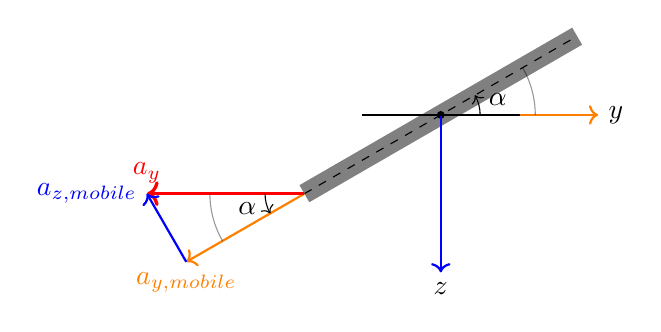
\begin{tikzpicture}
	\newcommand{\cosAngle}{0.866}
	\newcommand{\sinAngle}{0.5}
	\newcommand{\sideLength}{2}
	\newcommand{\mobileLength}{4}
	\newcommand{\hlh}{\mobileLength/2}
	\newcommand{\mobileThickness}{0.25}
    	
	\coordinate (origo) at (0,0);
    	\coordinate (point_on_x) at (2,0);

	\coordinate (end_a_y) at (-\hlh - \sideLength*\cosAngle,-1);
	

   	\begin{scope}[rotate=30]
		\coordinate (end_a_y_mobile) at (-\hlh-\cosAngle*\sideLength,0);
		\coordinate (begin_a_y) at (-\hlh, 0);

    		\fill[gray] ($ (origo) + (-\hlh,-\mobileThickness/2) $) rectangle ($ (origo) + (\hlh,\mobileThickness/2) $);
		\draw[dashed, black] (-\hlh,0)--(\hlh,0);
		\coordinate (rotated) at (\hlh,0);
		 \draw[thick,orange,->] (begin_a_y)  -- (end_a_y_mobile) node (y_mobile)
		 [orange,below] {$a_{y, mobile}$}; \begin{scope}[rotate=-30]
			\draw[very thick,red,->] (-\hlh*\cosAngle,-1)  -- (end_a_y) node (y_real)
			[red,above] {$a_y$}; 
			\draw[thick,blue,->](end_a_y_mobile)
						--
						(-\hlh - \sideLength*\cosAngle,-1) node (z_mobile) [blue, left] {$a_{z,
						mobile}$};
		\end{scope}
	\end{scope}	
    	% draw axes
    	\fill[black] (origo) circle (0.05);
    	\draw[thick,orange,->] (origo) -- ++(2,0) node[black,right] {$y$};
    	\draw[thick,blue,->] (origo) -- ++(0,-2) node (mary) [black,below] {$z$};
   	\draw[thick] ($ (origo) + (-1,0) $) -- ($ (origo) + (1,0) $);

	% angle axes
	\tkzMarkAngle[fill= orange,size=1.2cm,opacity=.4](point_on_x,origo,rotated)
    	\pic [draw, ->, "$\alpha$", angle eccentricity=1.5] {angle =
    	point_on_x--origo--rotated};

	% angle vectors
	\tkzMarkAngle[fill=
	orange,size=1.2cm,opacity=.4](end_a_y,begin_a_y,end_a_y_mobile) \pic [draw, ->,
	"$\alpha$", angle eccentricity=1.5] {angle = end_a_y--begin_a_y--end_a_y_mobile};
  \end{tikzpicture}
        \caption{$a_y$ depending on Pitch}
    \end{minipage}% <- sonst wird hier ein Leerzeichen eingef�gt
    \hfill
    \begin{minipage}{0.5\textwidth}
        \centering
			\begin{align} 
				a_{z, handy} &= \tan(\alpha) \cdot {a_{y, handy}}\\
				a_y &= \frac{a_{y, handy}}{\cos(\alpha)}
			\end{align}
    \end{minipage}
\end{figure}

\begin{figure}[htb]
    \centering
    \begin{minipage}{0.5\textwidth}
        \centering
        \captionsetup{justification=centering}
          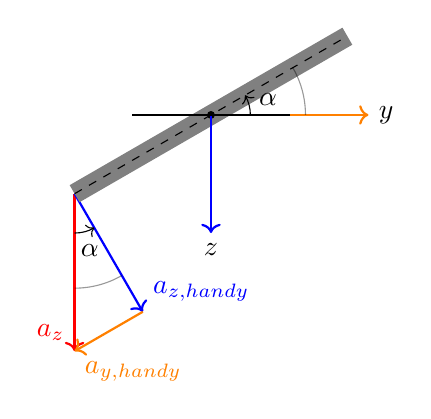
\begin{tikzpicture}
	\newcommand{\cosAngle}{0.866}
	\newcommand{\sinAngle}{0.5}
	\newcommand{\sideLength}{2}
	\newcommand{\handyLength}{4}
	\newcommand{\hlh}{\handyLength/2}
	\newcommand{\handyThickness}{0.25}
    	
	\coordinate (origo) at (0,0);
    	\coordinate (point_on_x) at (2,0);
	
	\begin{scope}[rotate=30]
		\coordinate (begin_a_z) at (-\hlh, 0);
	\end{scope}	

	\coordinate (end_a_y) at ($(begin_a_z)+(0,-\sideLength)$);
	\draw[thick,red,->] (begin_a_z) -- (end_a_y) node (y_real) [red,above left]
	{$a_z$}; 
	\begin{scope}[rotate=30]
		%\coordinate (end_a_z_handy) at ($(begin_a_z)+(0,-\sideLength)$);
		\coordinate (end_a_z_handy) at ($(begin_a_z)+(0,-\cosAngle*\sideLength)$);
	\end{scope}	
	\draw[thick,blue,->] (begin_a_z) -- (end_a_z_handy) node (z_handy) [blue,above
	right] {$a_{z, handy}$};

	\draw[thick,orange,->] (end_a_z_handy)  -- (end_a_y) node (y_handy)
	[orange,below right] {$a_{y, handy}$};

   	\begin{scope}[rotate=30]
		\coordinate (end_a_y_handy) at (-\hlh-\sideLength,0);
		%\coordinate (begin_a_z) at (-\hlh, 0);

    		\fill[gray] ($ (origo) + (-\hlh,-\handyThickness/2) $) rectangle ($ (origo) + (\hlh,\handyThickness/2) $);
		\draw[dashed, black] (-\hlh,0)--(\hlh,0);
		\coordinate (rotated) at (\hlh,0);
	\end{scope}	
    	% draw axes
    	\fill[black] (origo) circle (0.05);
    	\draw[thick,orange,->] (origo) -- ++(2,0) node[black,right] {$y$};
    	\draw[thick,blue,->] (origo) -- ++(0,-1.5) node (mary) [black,below] {$z$};
   	\draw[thick] ($ (origo) + (-1,0) $) -- ($ (origo) + (1,0) $);

	% angle axes
	\tkzMarkAngle[fill= orange,size=1.2cm,opacity=.4](point_on_x,origo,rotated)
    	\pic [draw, ->, "$\alpha$", angle eccentricity=1.5] {angle = point_on_x--origo--rotated};

	% angle vectors
	\tkzMarkAngle[fill=
	orange,size=1.2cm,opacity=.4](end_a_y,begin_a_z,end_a_z_handy) \pic [draw, ->,
	"$\alpha$", angle eccentricity=1.5] {angle = end_a_y--begin_a_z--end_a_z_handy};
  \end{tikzpicture}
        \caption{$a_z$ depending on Pitch}
    \end{minipage}% <- sonst wird hier ein Leerzeichen eingef�gt
    \hfill
    \begin{minipage}{0.5\textwidth}
        \centering
			\begin{align} 
				a_{y, handy} &= \tan(\alpha) \cdot a_{z, handy}\\ 
				a_z &= \frac{a_{z, handy}}{\cos(\alpha)}
			\end{align}
    \end{minipage}
\end{figure}

\FloatBarrier
\subsubsection{Acceleration depending on Roll}
\begin{figure}[htb]
    \centering
    \begin{minipage}{0.5\textwidth}
        \centering
        \captionsetup{justification=centering}
          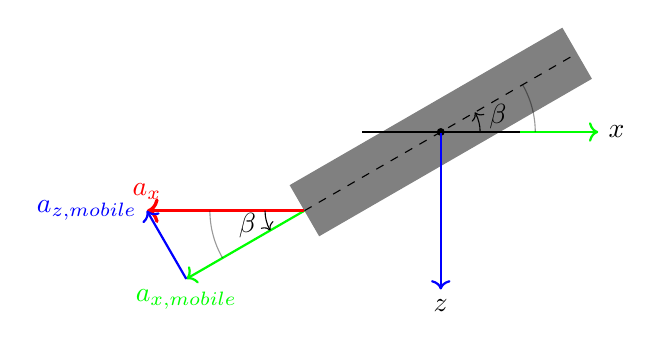
\begin{tikzpicture}
	\newcommand{\cosAngle}{0.866}
	\newcommand{\sinAngle}{0.5}
	\newcommand{\sideLength}{2}
	\newcommand{\mobileLength}{4}
	\newcommand{\hlh}{\mobileLength/2}
	\newcommand{\mobileThickness}{0.75}
    	
	\coordinate (origo) at (0,0);
    	\coordinate (point_on_x) at (2,0);

	\coordinate (end_a_y) at (-\hlh - \sideLength*\cosAngle,-1);
	

   	\begin{scope}[rotate=30]
		\coordinate (end_a_y_mobile) at (-\hlh-\cosAngle*\sideLength,0);
		\coordinate (begin_a_y) at (-\hlh, 0);

    		\fill[gray] ($ (origo) + (-\hlh,-\mobileThickness/2) $) rectangle ($ (origo) + (\hlh,\mobileThickness/2) $);
		\draw[dashed, black] (-\hlh,0)--(\hlh,0);
		\coordinate (rotated) at (\hlh,0);
		 \draw[thick,green,->] (begin_a_y)  -- (end_a_y_mobile) node (y_mobile)
		 [green,below] {$a_{x, mobile}$}; \begin{scope}[rotate=-30]
			\draw[very thick,red,->] (-\hlh*\cosAngle,-1)  -- (end_a_y) node (y_real)
			[red,above] {$a_x$}; 
			\draw[thick,blue,->](end_a_y_mobile)
						--
						(-\hlh - \sideLength*\cosAngle,-1) node (z_mobile) [blue, left] {$a_{z,
						mobile}$};
		\end{scope}
	\end{scope}	
    	% draw axes
    	\fill[black] (origo) circle (0.05);
    	\draw[thick,green,->] (origo) -- ++(2,0) node[black,right] {$x$};
    	\draw[thick,blue,->] (origo) -- ++(0,-2) node (mary) [black,below] {$z$};
   	\draw[thick] ($ (origo) + (-1,0) $) -- ($ (origo) + (1,0) $);

	% angle axes
	\tkzMarkAngle[fill= green,size=1.2cm,opacity=.4](point_on_x,origo,rotated)
    	\pic [draw, ->, "$\beta$", angle eccentricity=1.5] {angle =
    	point_on_x--origo--rotated};

	% angle vectors
	\tkzMarkAngle[fill=
	green,size=1.2cm,opacity=.4](end_a_y,begin_a_y,end_a_y_mobile) \pic [draw, ->,
	"$\beta$", angle eccentricity=1.5] {angle = end_a_y--begin_a_y--end_a_y_mobile};
  \end{tikzpicture}
        \caption{$a_x$ depending on Roll}
    \end{minipage}% <- sonst wird hier ein Leerzeichen eingef�gt
    \hfill
    \begin{minipage}{0.5\textwidth}
        \centering
			\begin{align} 
				a_{x, handy} &= \tan(\beta) \cdot {a_{x, handy}}\\
				a_x &= \frac{a_{x, handy}}{\cos(\beta)}
			\end{align}
    \end{minipage}
\end{figure}

\begin{figure}[htb]
    \centering
    \begin{minipage}{0.5\textwidth}
        \centering
        \captionsetup{justification=centering}
        \input{res/mathstuff/zRoll.tex}
        \caption{$a_z$ depending on Roll}
    \end{minipage}% <- sonst wird hier ein Leerzeichen eingef�gt
    \hfill
    \begin{minipage}{0.5\textwidth}
        \centering
			\begin{align} 
				a_{x, handy} &= \tan(\beta) \cdot a_{z, handy}\\ 
				a_z &= \frac{a_{z, handy}}{\cos(\alpha)}
			\end{align}
    \end{minipage}
\end{figure}

\FloatBarrier
\subsubsection{Acceleration depending on Azimuth}

\begin{figure}[htb]
    \centering
    \begin{minipage}{0.5\textwidth}
        \centering
        \captionsetup{justification=centering}
          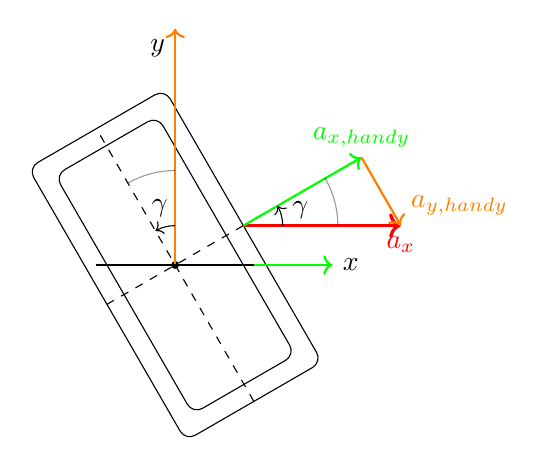
\begin{tikzpicture}
	\newcommand{\cosAngle}{0.866}
	\newcommand{\sinAngle}{0.5}
	\newcommand{\sideLength}{2}
	\newcommand{\handyLength}{4}
	\newcommand{\hlh}{\handyLength/2}
	\newcommand{\handyWidth}{2}
	\newcommand{\hwh}{\handyWidth/2}
	\newcommand{\padding}{0.25}

	\begin{scope}[rotate=120]
		\draw[rounded corners] (-\hlh,-\hwh) rectangle (\hlh,\hwh);
		\draw[rounded corners] (-\hlh+\padding,-\hwh+\padding) rectangle (\hlh-\padding,\hwh-\padding);
		\draw[dashed, black] (-\hlh,0)--(\hlh,0);
		\draw[dashed, black] (0,-\hwh)--(0,\hwh);
		\coordinate (begin_a_x) at (0, -\hwh);
	\end{scope}
	
	\coordinate (end_a_x) at ($(begin_a_x)+(\sideLength,0)$);
	\draw[very thick,red,->] (begin_a_x)  -- (end_a_x) node (x_real) [red,below] {$a_x$}; 

	\coordinate (end_a_x_handy) at ($(begin_a_x)+(\cosAngle*\cosAngle*\sideLength,\sinAngle*\cosAngle*\sideLength)$);
	\draw[thick,green,->] (begin_a_x)  -- (end_a_x_handy) node (x_handy) [green,above] {$a_{x, handy}$};
	
	\draw[thick,orange,->] (end_a_x_handy) -- (end_a_x) node (y_handy) [orange,above right] {$a_{y, handy}$};

	\begin{scope}[rotate=30]
		\coordinate (rotated) at (0,2);
	\end{scope}
    	
	\coordinate (origo) at (0,0);
    	\coordinate (point_on_z) at (0,2);

	\coordinate (end_a_y) at (-\hlh - \sideLength*\cosAngle,-1);

    	% draw axes
    	\fill[black] (origo) circle (0.05);
    	\draw[thick,green,->] (origo) -- ++(2,0) node[black,right] {$x$};
    	\draw[thick,orange,->] (origo) -- ++(0,3) node (mary) [black,below left] {$y$};
   	\draw[thick] ($ (origo) + (-1,0) $) -- ($ (origo) + (1,0) $);

	% angle axes
	\tkzMarkAngle[fill= blue,size=1.2cm,opacity=.4](point_on_z,origo,rotated)
    	\pic [draw, ->, "$\gamma$", angle eccentricity=1.5] {angle =
    	point_on_z--origo--rotated};

	% angle vectors
	\tkzMarkAngle[fill=
	blue,size=1.2cm,opacity=.4](end_a_x,begin_a_x,end_a_x_handy) \pic [draw, ->,
	"$\gamma$", angle eccentricity=1.5] {angle = end_a_x--begin_a_x--end_a_x_handy};
  \end{tikzpicture}
        \caption{$a_x$ depending on Azimuth}
    \end{minipage}% <- sonst wird hier ein Leerzeichen eingef�gt
    \hfill
    \begin{minipage}{0.5\textwidth}
        \centering
			\begin{align} 
				a_{y, handy} &= \tan(\gamma) \cdot {a_{x, handy}}\\
				a_x &= \frac{a_{x, handy}}{\cos(\gamma)}
			\end{align}
    \end{minipage}
\end{figure}

\begin{figure}[htb]
    \centering
    \begin{minipage}{0.5\textwidth}
        \centering
        \captionsetup{justification=centering}
          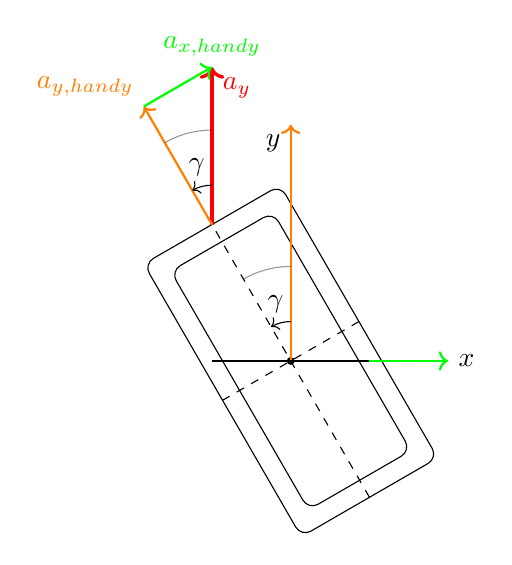
\begin{tikzpicture}
	\newcommand{\cosAngle}{0.866}
	\newcommand{\sinAngle}{0.5}
	\newcommand{\sideLength}{2}
	\newcommand{\handyLength}{4}
	\newcommand{\hlh}{\handyLength/2}
	\newcommand{\handyWidth}{2}
	\newcommand{\hwh}{\handyWidth/2}
	\newcommand{\padding}{0.25}

	\begin{scope}[rotate=120]
		\draw[rounded corners] (-\hlh,-\hwh) rectangle (\hlh,\hwh);
		\draw[rounded corners] (-\hlh+\padding,-\hwh+\padding) rectangle (\hlh-\padding,\hwh-\padding);
		\draw[dashed, black] (-\hlh,0)--(\hlh,0);
		\draw[dashed, black] (0,-\hwh)--(0,\hwh);
		\coordinate (begin_a_y) at (\hlh, 0);
	\end{scope}
	
	\coordinate (end_a_y) at ($(begin_a_y)+(0, \sideLength)$);
	\draw[very thick,red,->] (begin_a_y)  -- (end_a_y) node (x_real) [red,below right] {$a_y$}; 

	\coordinate (end_a_y_handy) at ($(begin_a_y)+(-\sinAngle*\cosAngle*\sideLength,\cosAngle*\cosAngle*\sideLength)$);
	\draw[thick,orange,->] (begin_a_y)  -- (end_a_y_handy) node (y_handy) [orange,above left] {$a_{y, handy}$};
	
	\draw[thick,green,->] (end_a_y_handy) -- (end_a_y) node (y_handy) [green,above] {$a_{x, handy}$};

	\begin{scope}[rotate=30]
		\coordinate (rotated) at (0,2);
	\end{scope}
    	
	\coordinate (origo) at (0,0);
    	\coordinate (point_on_z) at (0,2);

    	% draw axes
    	\fill[black] (origo) circle (0.05);
    	\draw[thick,green,->] (origo) -- ++(2,0) node[black,right] {$x$};
    	\draw[thick,orange,->] (origo) -- ++(0,3) node (mary) [black,below left] {$y$};
   	\draw[thick] ($ (origo) + (-1,0) $) -- ($ (origo) + (1,0) $);

	% angle axes
	\tkzMarkAngle[fill= blue,size=1.2cm,opacity=.4](point_on_z,origo,rotated)
    	\pic [draw, ->, "$\gamma$", angle eccentricity=1.5] {angle =
    	point_on_z--origo--rotated};

	% angle vectors
	\tkzMarkAngle[fill=	blue,size=1.2cm,opacity=.4](end_a_y,begin_a_y,end_a_y_handy) 
	\pic [draw, ->,"$\gamma$", angle eccentricity=1.5] {angle = end_a_y--begin_a_y--end_a_y_handy};
  \end{tikzpicture}
        \caption{$a_y$ depending on Azimuth}
    \end{minipage}% <- sonst wird hier ein Leerzeichen eingef�gt
    \hfill
    \begin{minipage}{0.5\textwidth}
        \centering
			\begin{align} 
				a_{x, handy} &= \tan(\gamma) \cdot a_{y, handy}\\ 
				a_y &= \frac{a_{y, handy}}{\cos(\gamma)}
			\end{align}
    \end{minipage}
\end{figure}

\FloatBarrier
\section{Recognition of Gestures}
The system recognizes two kind of gestures (see also
\ref{fig:gesturesToRecognize}):
\begin{itemize}
  \item A circle that starts from the bottom and runs clockwise
  \item A circle that starts from the bottom and runs counter-clockwise
\end{itemize}
The first gesture is used to mark an item as ``added to cart'' while the second
one serves to switch through the items on the shopping list.

\begin{figure}[h]
\captionsetup{justification=centering}
\begin{subfigure}{0.475\textwidth}
\includegraphics[width=\textwidth]{res/gestures/addToCart.png}
\caption{Add Item to Cart}
\label{fig:gestureAdd}
\end{subfigure} \hspace{0.05\textwidth}
\begin{subfigure}{0.475\textwidth}
\includegraphics[width=\textwidth]{res/gestures/removeFromCart.png}
\caption{Switch Item}
\label{fig:gestureRemove}
\end{subfigure}
\caption{Gestures to Recognize}
\label{fig:gesturesToRecognize}
\end{figure}

\begin{figure}
\centering
\captionsetup{justification=centering}
\begin{tikzpicture}
\begin{axis}[
  id=Measured accelerations,
			width=0.9\textwidth,height=0.3\textheight,
			%title={Measured Accelerations},
    		grid =both,
    		minor x tick num = 1,
    		minor y tick num = 1,
			xlabel={Measurement Point},
			ylabel={Acceleration Values [$\frac{m}{s^2}$]}, ymin=-15, xmin=0,
			xmax=250, legend style={ at={(0,1)}, anchor=north west}]
\addplot [mark=none, blue, thick] 
		plot table [x=Point, y=a_{x}]{res/gestures/finalExcel.csv};
\addlegendentry{$a_x$}
\addplot [mark=none, ForestGreen, thick] 
		plot table [x=Point, y=a_{z}]{res/gestures/finalExcel.csv};
\addlegendentry{$a_z$}
\end{axis}
\end{tikzpicture}
\caption{Calculated Values $a_x$ and $a_z$ for two Circles}
\label{fig:finalAcc}
\end{figure}

\begin{figure}
\centering
\captionsetup{justification=centering}
\begin{tikzpicture}
\begin{axis}[
  id=Measured accelerations,
			width=0.9\textwidth,height=0.3\textheight,
			%title={Measured Accelerations},
    		grid =both,
    		minor x tick num = 1,
    		minor y tick num = 1,
			xlabel={Measurement Point},
			ylabel={Acceleration Values [$\frac{m}{s^2}$]}, ymin=-15, xmin=0,
			xmax=250, legend style={ at={(0,1)}, anchor=north west}] 
\addplot [mark=none, blue, thick] 
		plot table [x=Point, y=x]{res/gestures/kreis_flach_1.csv};
\addlegendentry{$a_x$}
\addplot [mark=none, magenta, thick] 
		plot table [x=Point, y=y]{res/gestures/kreis_flach_1.csv};
\addlegendentry{$a_y$}
\addplot [mark=none, ForestGreen, thick] 
		plot table [x=Point, y=z]{res/gestures/kreis_flach_1.csv};
\addlegendentry{$a_z$}
\end{axis}
\end{tikzpicture}
\caption{Calculated Values $a_x$ and $a_z$ for two Circles}
\label{fig:finalAcc}
\end{figure}


\FloatBarrier
\section{Result}
\subsection{User Manual}


\begin{figure}[h]
\captionsetup{justification=centering}
\begin{subfigure}{0.475\textwidth} 
\centering 
\includegraphics[height= 0.35\textheight]{res/usermanual/startApp.png}
\caption{Start}
\label{fig:start}
\end{subfigure} \hspace{0.05\textwidth}
\begin{subfigure}{0.475\textwidth}
\centering 
\includegraphics[height= 0.35\textheight]{res/usermanual/initialShoppinglist.png}
\caption{Initial Shoppinglist}
\label{fig:initial}
\end{subfigure}
\caption{Initial State after Starting the App}
\label{fig:initialState}
\end{figure}


\begin{figure}[h]
\captionsetup{justification=centering}
\begin{subfigure}{0.475\textwidth} 
\centering 
\includegraphics[height= 0.35\textheight]{res/usermanual/firstItemChecked.png}
\caption{First Item Checked Off}
\label{fig:firstItemChecked}
\end{subfigure} \hspace{0.05\textwidth}
\begin{subfigure}{0.475\textwidth}
\centering 
\includegraphics[height= 0.35\textheight]{res/usermanual/circleRecognized.png}
\caption{Feedback Circle Recognized}
\label{fig:initial}
\end{subfigure}
\caption{Check Off Items}
\label{fig:checkItems}
\end{figure}


\begin{figure}[h]
\captionsetup{justification=centering}
\begin{subfigure}{0.475\textwidth}
\centering 
\includegraphics[height= 0.35\textheight]{res/usermanual/notswitched.png}
\caption{Shoppinglist before Switching}
\label{fig:beforeSwitching}
\end{subfigure} \hspace{0.05\textwidth}
\begin{subfigure}{0.475\textwidth}
\centering
\includegraphics[height= 0.35\textheight]{res/usermanual/switched.png}
\caption{Shoppinglist after Switching}
\label{fig:afterSwitching}
\end{subfigure}
\caption{Switch Items}
\label{fig:checkItems}
\end{figure}

\FloatBarrier

\subsection{Conclusion}



\input{contents/Registers.tex}
 
\end{document}
